\subsubsection{Class Diagram}

\begin{figure}[H]
    \centering
    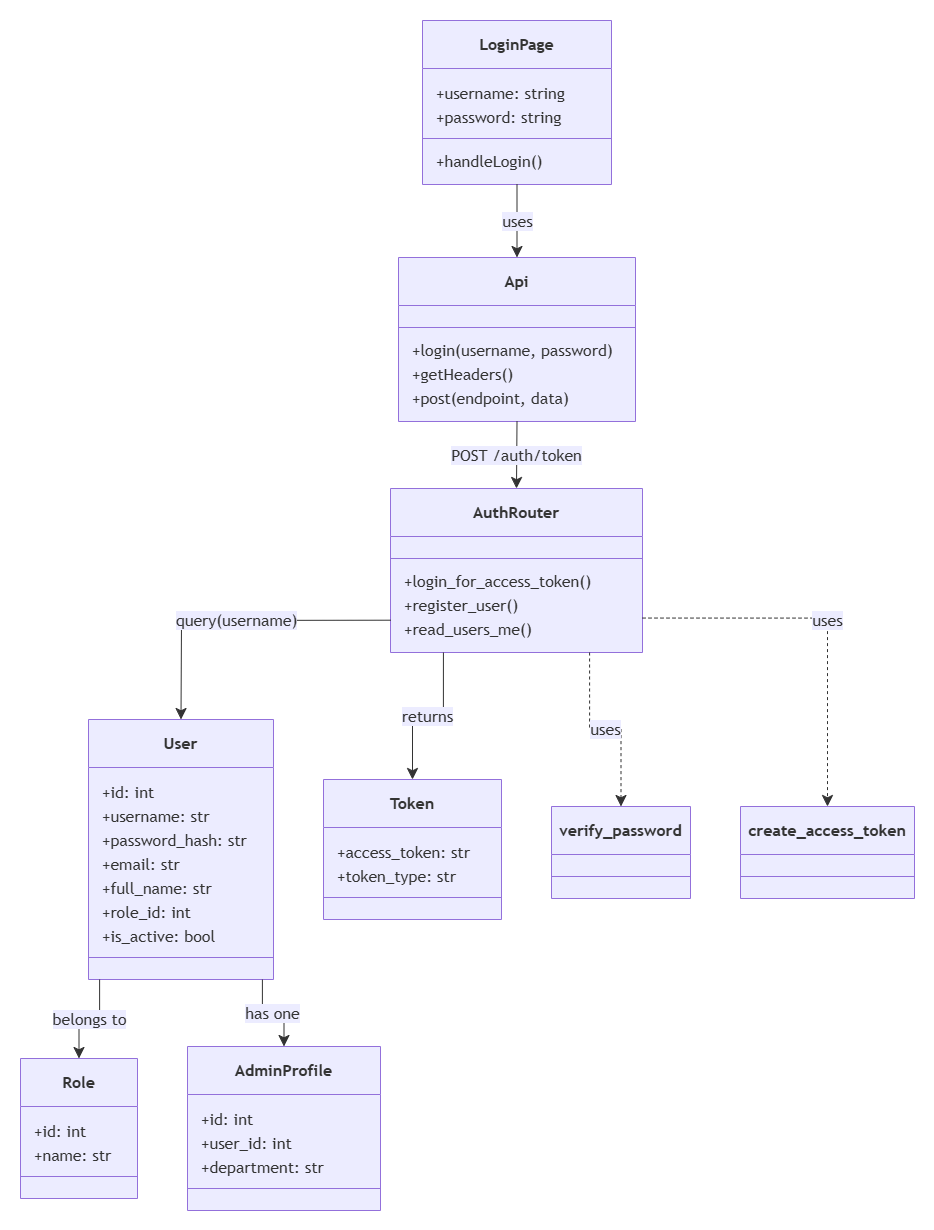
\includegraphics[width=\textwidth]{figures/design/admin/admin_login_class.png}
    \caption{Admin Login Class Diagram}
    \label{fig:admin_login_class_diagram}
\end{figure}

\subsubsection{Class Specification}

\begingroup
\small
\setlength{\tabcolsep}{3pt}
\TableStart{|>{\raggedright\arraybackslash}p{0.15\textwidth}|>{\raggedright\arraybackslash}p{0.31\textwidth}|>{\raggedright\arraybackslash}p{0.14\textwidth}|>{\raggedright\arraybackslash}p{0.25\textwidth}|}
\textbf{Class} & \textbf{Attributes / Methods} & \textbf{Type} & \textbf{Description} \\
\hline
LoginPage & username, password, handleLogin() & state / action & UI component that collects admin credentials and invokes the API service. \\
\hline
Api & login(username, password), getHeaders(), post(endpoint, data) & service / helper & Sends authentication request to \texttt{POST /auth/token}, stores bearer token, and builds request headers for protected calls. \\
\hline
AuthRouter & login\_for\_access\_token(), register\_user(), read\_users\_me() & controller / route & Handles auth endpoints, verifies credentials, issues bearer tokens, and returns authenticated user details. \\
\hline
User & id, username, password\_hash, email, full\_name, role\_id, is\_active & entity & Database user entity carrying credentials, role assignment, and active status. \\
\hline
Role & id, name & entity & Role entity defining access levels such as \texttt{ADMIN}, \texttt{OWNER}, \texttt{JOCKEY}, \texttt{REFEREE}, and \texttt{SPECTATOR}. \\
\hline
Token & access\_token, token\_type & DTO & Authentication response containing bearer token data after successful login. \\
\hline
AdminProfile & id, user\_id, department & entity & Admin-specific profile information associated with a User account. \\
\TableFinish{Admin Login class specification}{tab:admin_login_class_spec}
\endgroup
